

\chapter{Coding strategies}
This chapter is all about how to alter our predictors and outcomes to make regression models give us the information we need to know.
\section{Centering}
The most basic transformation of a variable is to add or subtract something from it. An important example of this is to center a variable. This is also called de-meaning a variable (but I prefer "centering"). Centering a variable is the simple procedure of taking a variable and subtracting its mean value.
\begin{equation}
x_i^{*}=x_i-\bar{x}
\end{equation}
This does powerful things for regressions and it makes your life easier. The benefits include making your intercept more interpretable and understanding complex coding schemes such as interactions much easier. It should be noted that centering will not change your slopes or the standard errors of your slopes. It will change your intercept and the standard error of your intercept.

It works by moving the $y$-intercept to the mean of your predictor. Since the intercept is always when your predictor(s) are 0, you make 0 the mean when you subtract it, see Figure~\ref{fig:centering_fit}.
\begin{figure}
   \centering
   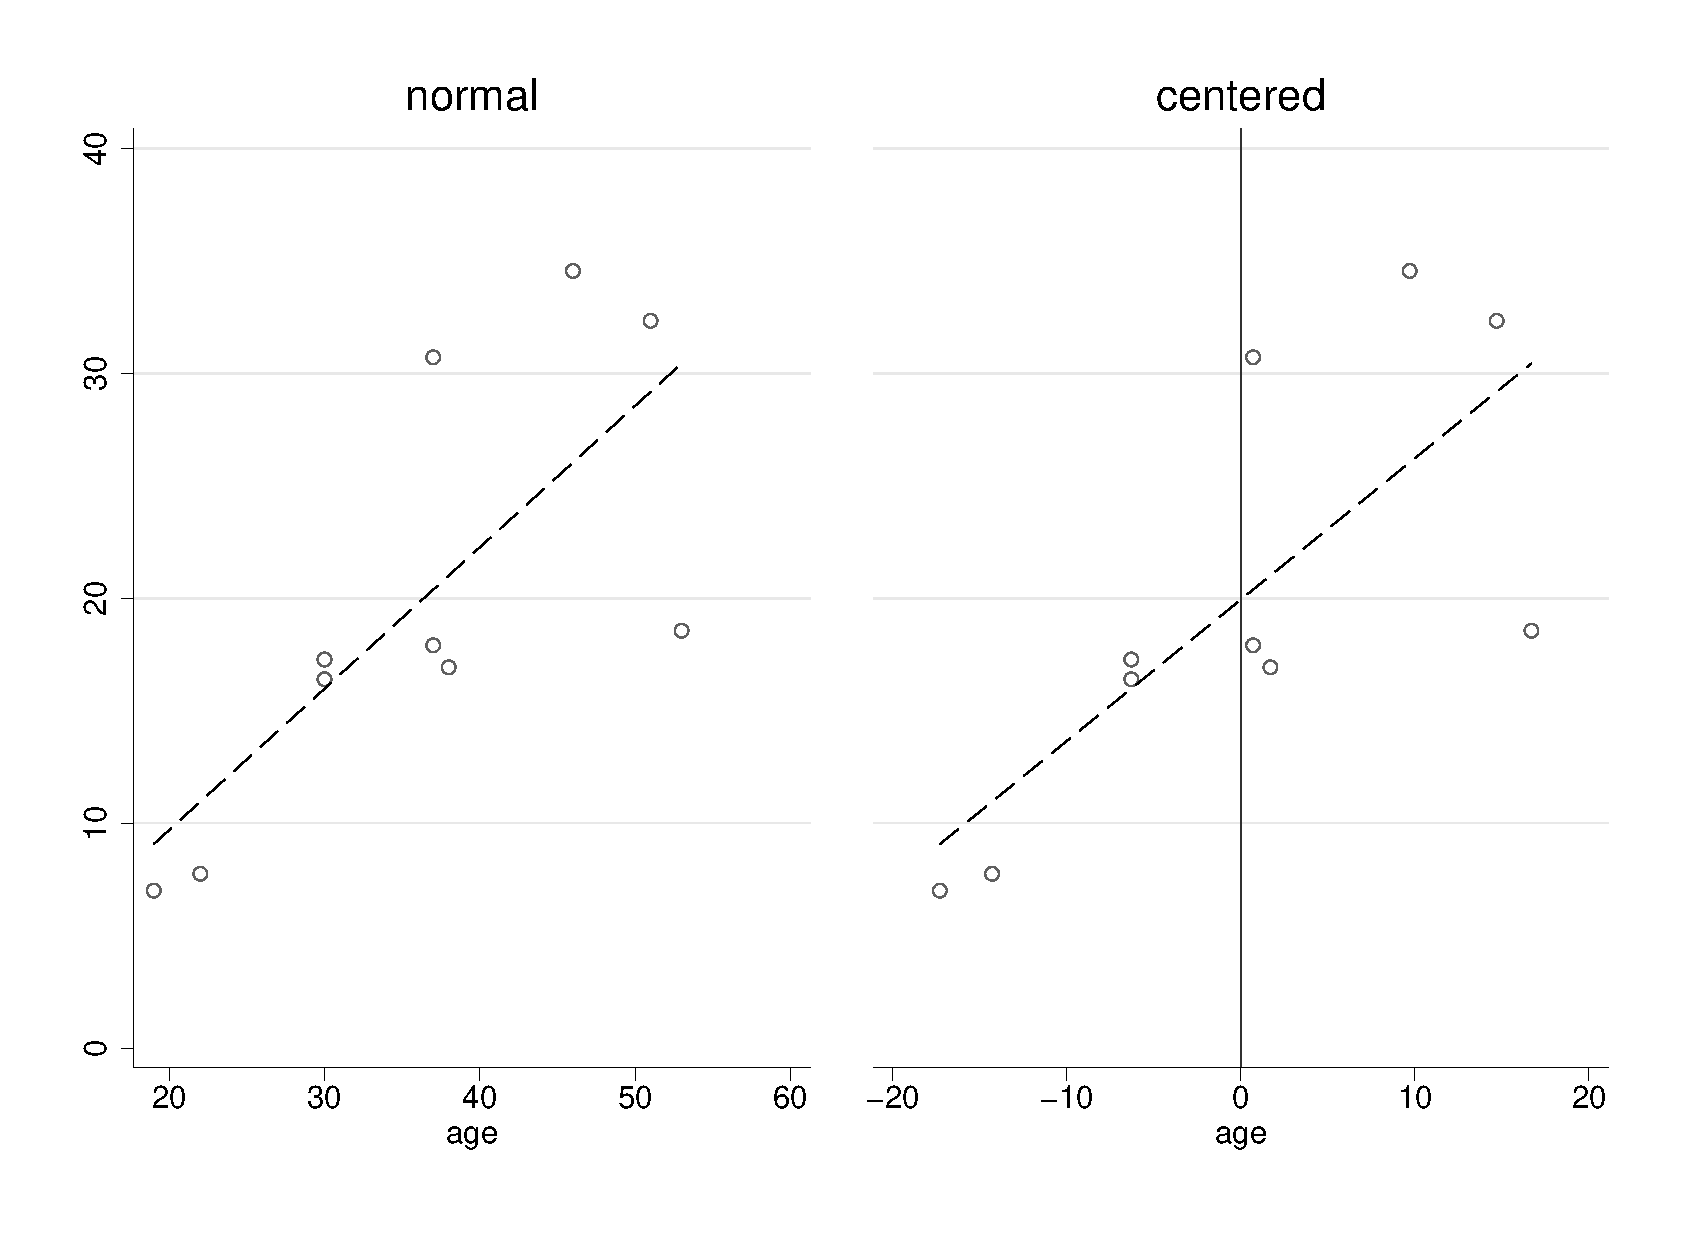
\includegraphics[angle=0,
           width=.75\textwidth]{centering_fit.eps}
   \caption{Illustration of centering}
  \label{fig:centering_fit}
\end{figure}
Centering can be done in models with a single variable or with many variables.

To understand what centering does, consider Model 3 from Table~\ref{tab:wagereg_all}:
\[
\hat{y}_i=\beta_0+\beta_1edu_i+\beta_2age_i+\beta_3female_i
\]
We know that $\beta_1$ is the effect of a single year of education on wages, $\beta_2$ is the effect of a single year of age on wages, and $\beta_3$ is the difference between females and males. What does $\beta_0$ mean again? It's the (average) value of $wage$ when $edu$, $age$, and $female$, all equal zero. Consider the models in Table~\ref{tab:wagecenter}, which use more data than the wage models in the other tables. In Model 1, none of the variables are centered.  So, according to this model, the intercept tells us that uneducated babies who are male make -4.651 dollars an hour. This doesn't make sense on many levels.
\begin{table}[htbp]\centering
\caption{Models predicting age with different centering strategies
\label{tab:wagecenter}}
\begin{tabular}{lccc}
\hline
Coefficients&Model 1&Model 2&Model 3 \\
\hline
edu &    0.930***&    0.930***&    0.930***\\
      &   (0.034)  &   (0.034)  &   (0.034)  \\
age     &    0.261***&    0.261***&    0.261***\\
      &   (0.009)  &   (0.009)  &   (0.009)  \\
female   &   -3.474***&   -3.474***&   -3.474***\\
      &   (0.207)  &   (0.207)  &   (0.207)  \\
Intercept    &   -4.651***&    5.006***&   17.289***\\
      &   (0.597)  &   (0.474)  &   (0.147)  \\
\hline
\multicolumn{4}{l}{Model Statistics} \\
\hline
$N$ 							&  3997.000  &  3997.000  &  3997.000  \\
$F$ 							&   590.668  &   590.668  &   590.668  \\
$R^2$ 						&    0.307  &    0.307  &    0.307  \\
$df$ Regression 			&    3.000  &    3.000  &    3.000  \\
Sum of Squares Regression 	&  75828.174  &  75828.174  &  75828.174  \\
$df$ Error 					&  3993.000  &  3993.000  &  3993.000  \\
Sum of Squares Error 		& 170869.757  & 170869.757  & 170869.757  \\
\hline
\multicolumn{4}{l}{Model 2: age centered, Model 3: edu and age centered.} \\
\multicolumn{4}{l}{$SE$s in parentheses, $***p<0.001$} \\
\hline
\end{tabular}
\end{table}
We now move to Model 2, where we have centered age. Now the intercept tells us that an {\it averaged aged} male with no education can expect to make about 5 dollars an hour. This is plausible. Next, in Model 3, we also center education. Now, an averaged aged male with an average number of years of education makes 17.30 an hour. Notice that in each case, while the intercept changed, the standard error of the intercept kept getting smaller and smaller. No other numbers in the table changed.

The standard error of the intercept gets smaller because the variance of any predicted value is always lowest at the mean. The reason for this is because the variance of any predicted value of $y$ based on some value of $x$, say $x_0$, is equation~\eqref{eq:varfit}
\[
\mbox{var}\left(\hat{y}_0\right)=\left(\frac{\sigma^2}{N}+\frac{\left(x_0-\bar{x}\right)^2\sigma^2}{\sum_{i=1}^N\left(x_i-\bar{x}\right)^2}\right)\sigma^2
\]
and that fraction to the right gets smaller the closer the value is to the mean of $x$. This gets reflected in the smaller standard error of the intercept.
\begin{figure}
   \centering
   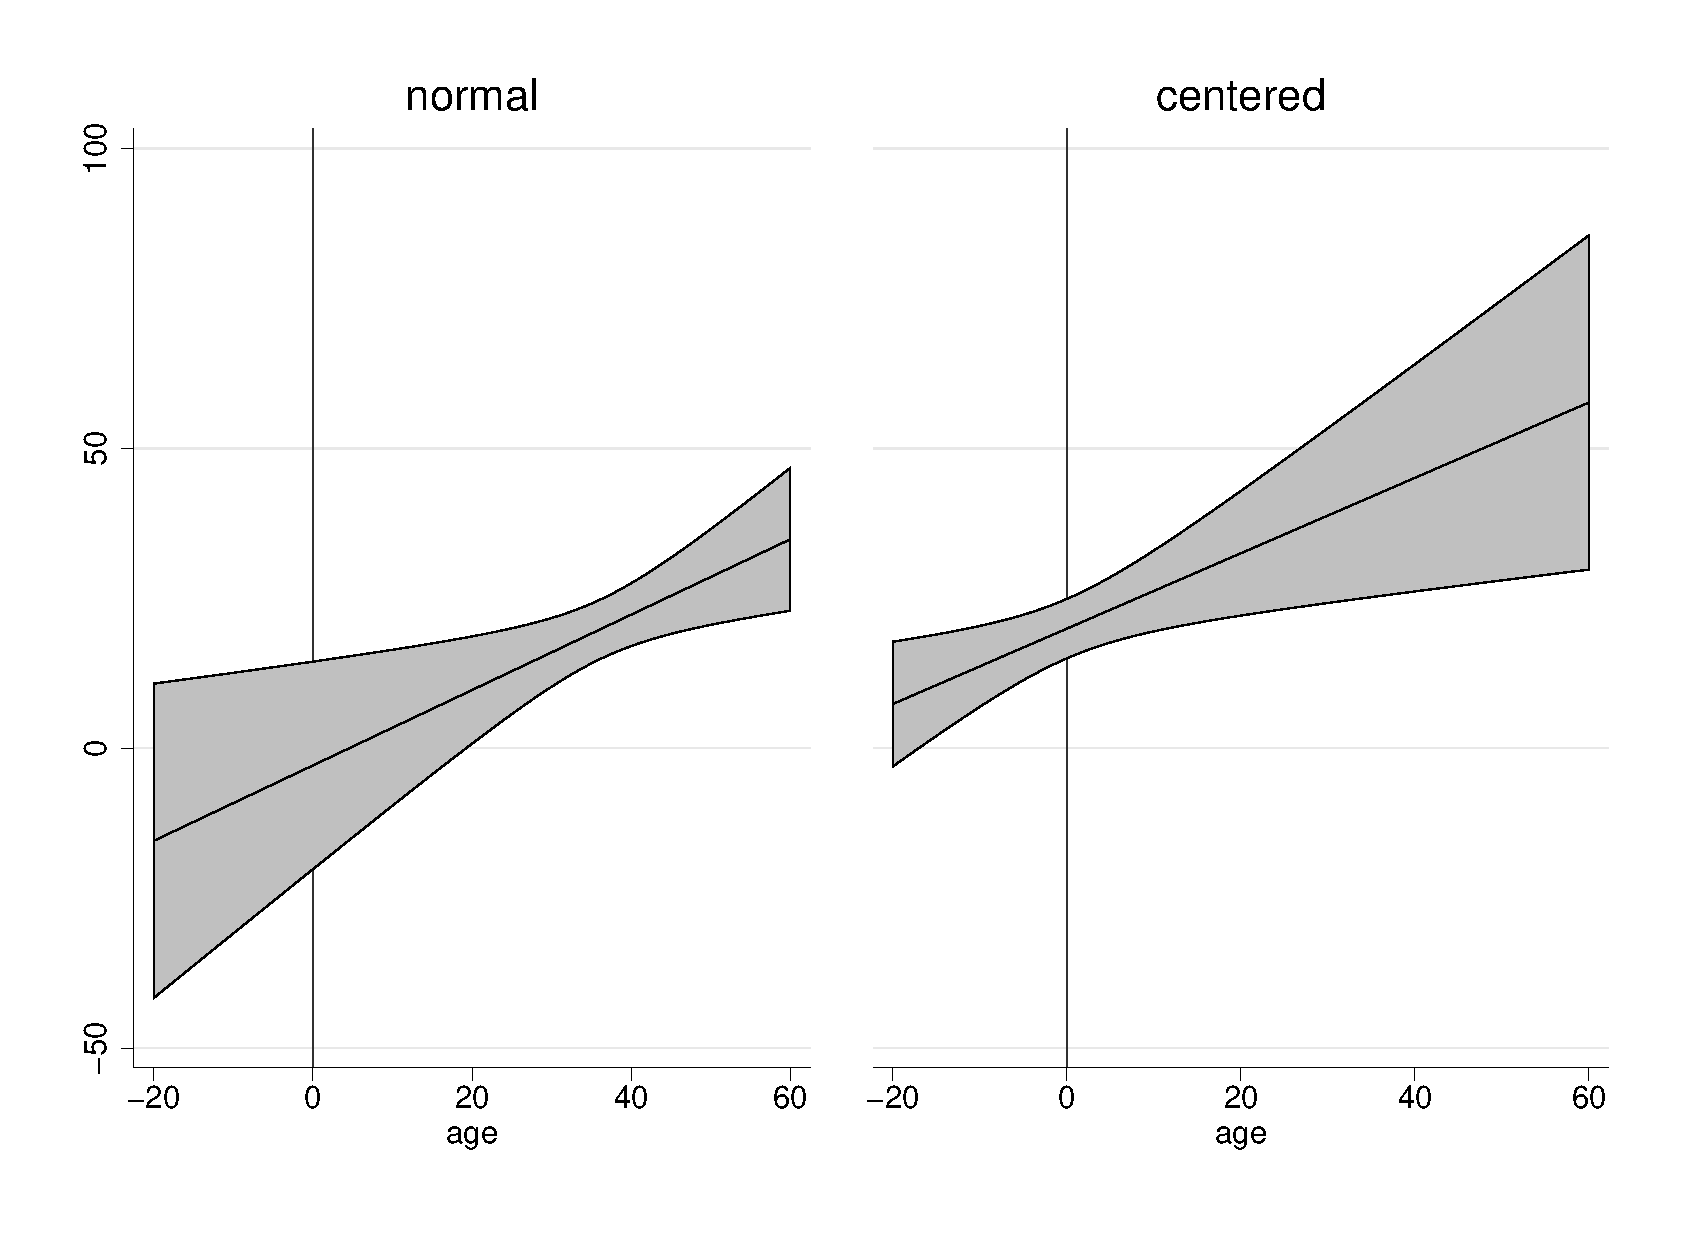
\includegraphics[angle=0,
           width=.75\textwidth]{centering_fitci.eps}
   \caption{Confidence interval of regression line}
  \label{fig:centering_fitci}
\end{figure}
We can see this in the bivariate case by looking at Figure~\ref{fig:centering_fitci}. Note how the confidence intervals are small around the mean of the distribution of the predictor. Centering moves the intercept to this point of small(er) variance. Centering is a good practice for building a good "reference" statistic.

\begin{table}[htbp]\centering
\caption{ Wage models with different age and education units
\label{tab:wagereg_alt}}
\begin{tabular}{lccc}
\hline
Coefficients&Model 1&Model 2&Model 3 \\
\hline
edu &    0.930***&    0.930***&    2.823***\\
      &   (0.034)  &   (0.034)  &   (0.104)  \\
age     &    0.261***&    2.613***&    2.613***\\
      &   (0.009)  &   (0.087)  &   (0.087)  \\
female   &   -3.474***&   -3.474***&   -3.474***\\
      &   (0.207)  &   (0.207)  &   (0.207)  \\
Intercept    &   -4.651***&   -4.651***&    7.632***\\
      &   (0.597)  &   (0.597)  &   (0.353)  \\
\hline
\multicolumn{4}{l}{Model Statistics} \\
\hline
$N$ &  3997.000  &  3997.000  &  3997.000  \\
$F$ &   590.668  &   590.668  &   590.668  \\
$R^2$ &    0.307  &    0.307  &    0.307  \\
$df$ Regression &    3.000  &    3.000  &    3.000  \\
Sum of Squares Regression 	 &  75828.174  &  75828.174  &  75828.174  \\
$df$ Error 		 &  3993.000  &  3993.000  &  3993.000  \\
Sum of Squares Error 	 & 170869.757  & 170869.757  & 170869.757  \\
\hline
\multicolumn{4}{l}{Model 2: age in 10 year units.} \\
\multicolumn{4}{l}{Model 3: age in 10 year units and edu is standardized.} \\
\multicolumn{4}{l}{$SE$s in parentheses, $***p<0.001$} \\
\hline
\end{tabular}
\end{table}

\section{Changing the unit}

A regression slope always tells us the difference in the outcome based on a single-unit increase in the predictor. Sometimes, a single unit increase isn't meaningful. For example, take age. Your wage probably won't increase that much from year to year. According to Table~\ref{tab:wagecenter}, Model 1, it will increase by 26.1 cents a year. A more meaningful distinction would be 10 years of age.

To capture this, we could divide age by 10 and rerun the model. This would make $\beta_2=2.613$. By moving the decimal of the predictor left, we move the decimal of the slope (and standard error) to the right. Compare the effect of age in Models 1 and 2 in Table~\ref{tab:wagereg_alt}. Nothing else changes. It is good practice to keep your predictors in units to maximize the digits available in your tables.

\section{Standardization}

Another transformation is $z$-scoring. It is simply centering the predictor and dividing by the standard deviation of the predictor
\begin{equation}
x_i^{(z)}=\frac{x_i-\bar{x}}{s_x}
\end{equation}

Sometimes this is called standardization. This changes the units of the variable into "standard deviation" units. This also centers variables on their mean. The slope's interpretation is now that a one-unit increase in the predictor is "a standard deviation" increase. Compare the effect of education in Models 2 and 3 in Table~\ref{tab:wagereg_alt}. In Model 2, for every year of education, wages increase by 93 cents. In Model 3, we see that an increase of a standard deviation in education increases wages by about 2.82 dollars. Nothing else changes.


\section{Power Transformations}

Sometimes the data are not linear. They need to be linear for a regression to count. There are several ways to transform data. One is the Box-Cox family of transformations
\begin{equation}
x\rightarrow x^p\equiv\frac{x^p-1}{p}\forall p>0
\end{equation}
This gives us the various effects of squaring, etc. This is nice when we think that the effect of $x$ on $y$ is not constant (like it accelerates or decelerates). {\bf Be careful with squares, always graph out our predicted values to know what you are dealing with}.

Many people make the mistake that just because a square term is significant, it must mean a u-shaped relationship. That depends on the strength of the main effect (i.e., the effect of $x$) and the effect of the square (i.e., the effect of $x^2$). Figures~\ref{fig:square1} through~\ref{fig:square4} illustrate the differences.
\begin{figure}
   \centering
   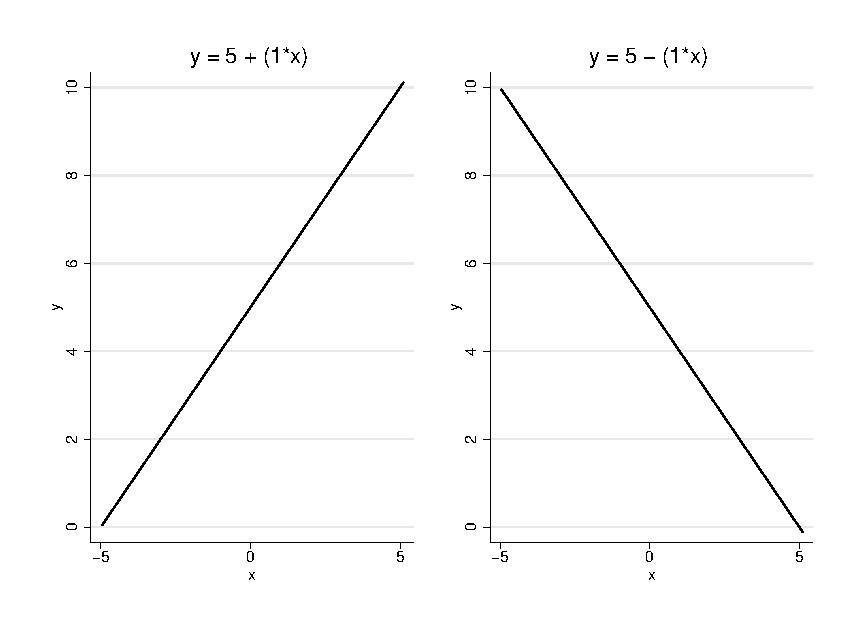
\includegraphics[angle=0,
           width=.75\textwidth]{square1.eps}
   \caption{Models without a quadratic relationships}
  \label{fig:square1}
\end{figure}
\begin{figure}
   \centering
   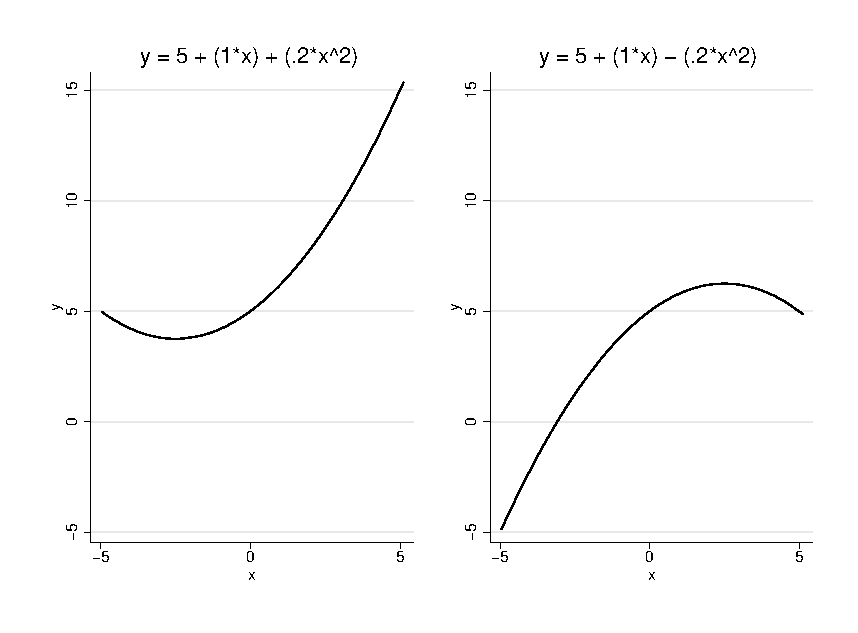
\includegraphics[angle=0,
           width=.75\textwidth]{square2.eps}
   \caption{Models with a positive relationship that accelerates (left) and one that decelerates (right)}
  \label{fig:square2}
\end{figure}
\begin{figure}
   \centering
   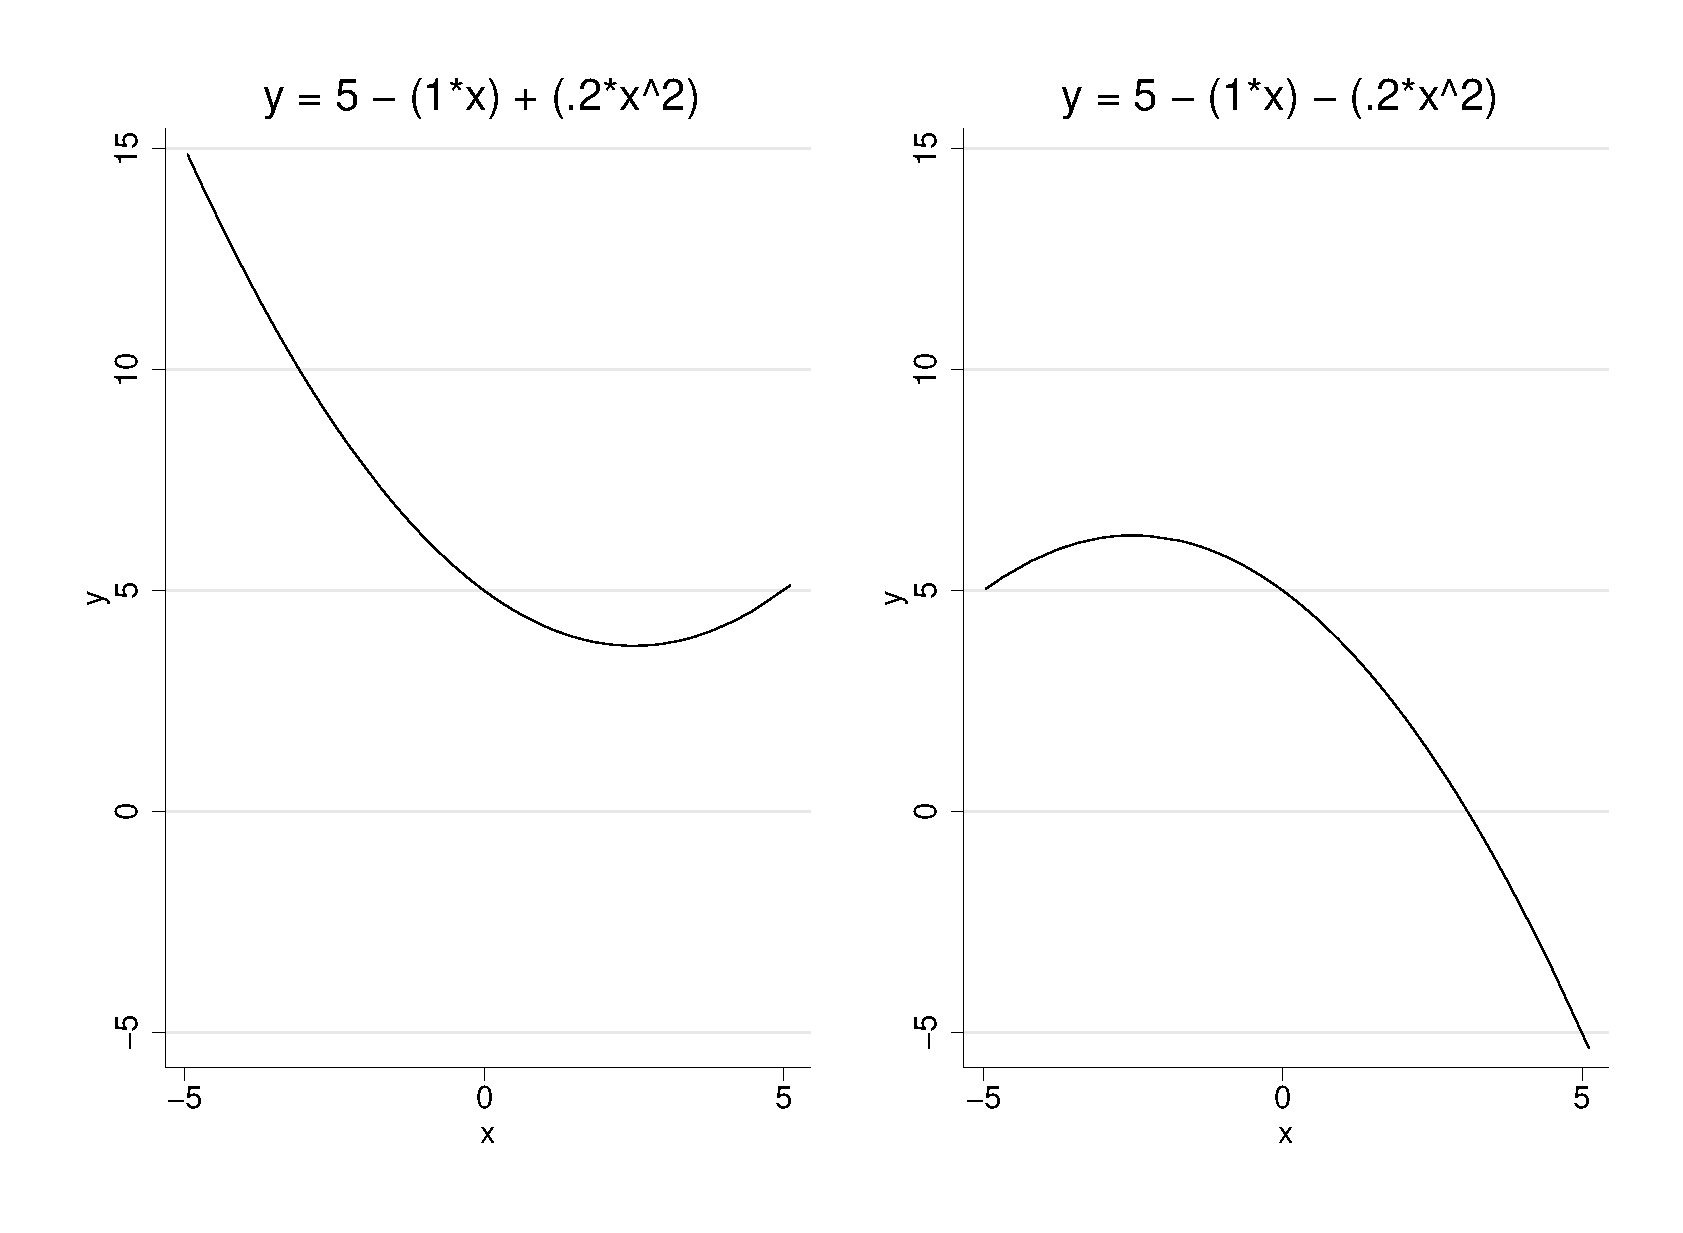
\includegraphics[angle=0,
           width=.75\textwidth]{square3.eps}
   \caption{Models with a negative relationship that decelerates (left) and one that accelerates (right)}
  \label{fig:square3}
\end{figure}
\begin{figure}
   \centering
   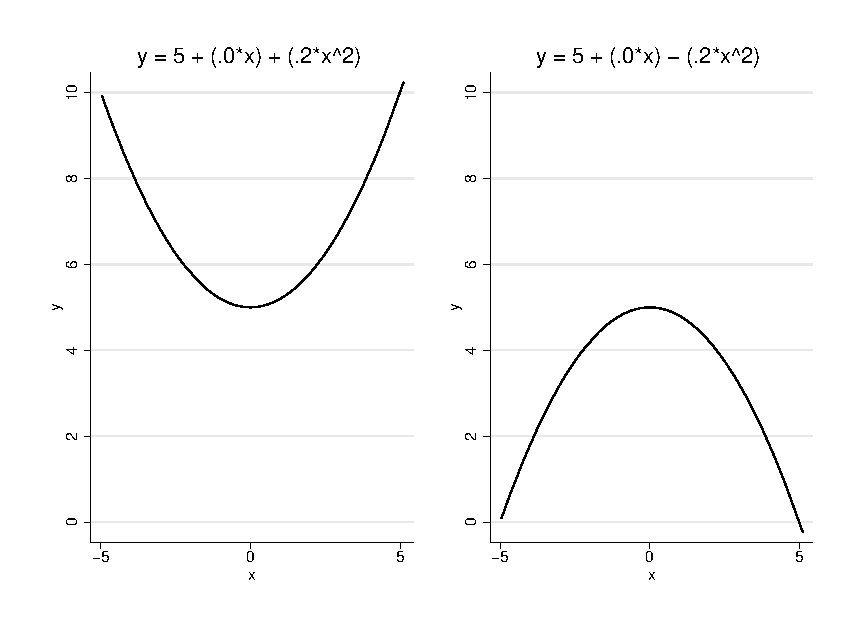
\includegraphics[angle=0,
           width=.75\textwidth]{square4.eps}
   \caption{Models without a main effect but a positive quadratic relationship (left) and a negative relationship (right)}
  \label{fig:square4}
\end{figure}
What can also be important is to know what the slope of the line is at any given point along the line. Let's take the function
\[
y=\beta_0-\beta_1x-\beta_2x^2
\]
\[
y=5-1x-0.2x^2
\]
What is the slope (or the slope of the tangent line) of this line at $x = 0.50$? Calculus gives us an easy formula for this
\begin{equation}
\frac{\partial y}{\partial x}|x=\beta_1+2\beta_2x
\end{equation}
for example, when x = 0.50,
\[
\frac{\partial y}{\partial x}|x=-1+2\left(-.2\right)x
\]
\[
\frac{\partial y}{\partial x}|x=-1+2\left(-.2\right)0.50
\]
\[
\frac{\partial y}{\partial x}|x=-1.2
\]
This is visualized in Figure~\ref{fig:calc}; notice the intercept for the tangent line is the same as the regression line.
\begin{figure}
   \centering
   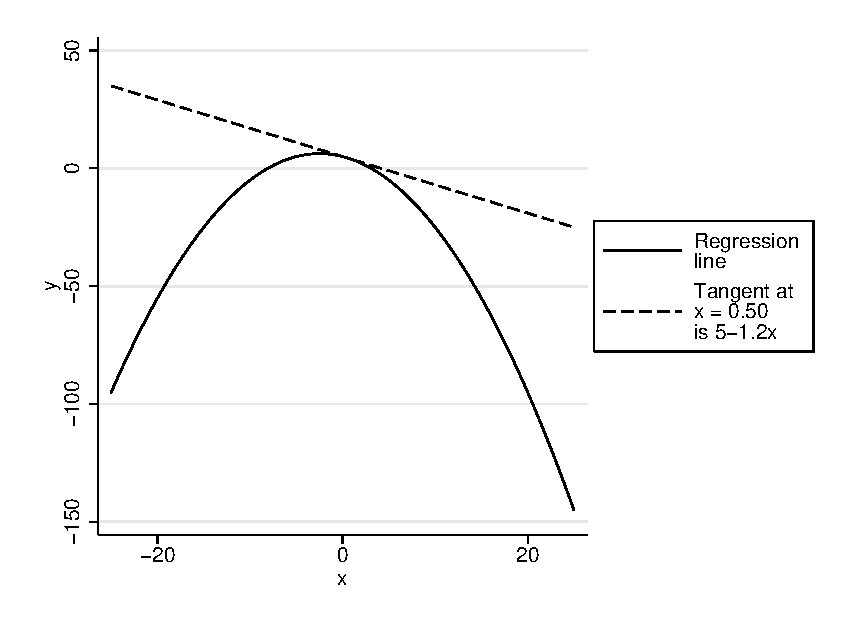
\includegraphics[angle=0,
           width=.75\textwidth]{calc.eps}
   \caption{Quadratic relationship with tangent}
  \label{fig:calc}
\end{figure}
\subsection{Logs}
\label{sec:logs}
A special case of a power transformation is the log. Figure~\ref{fig:ln} shows the natural log, $\mbox{ln}\left(x\right)$.
\begin{figure}
   \centering
   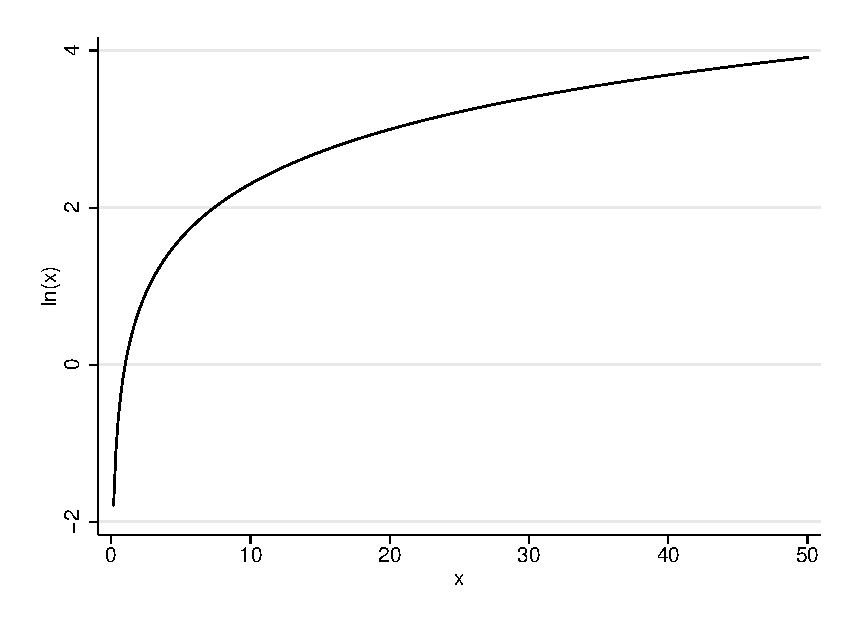
\includegraphics[angle=0,
           width=.75\textwidth]{ln.eps}
   \caption{ln($x$)}
  \label{fig:ln}
\end{figure}
This helps tone down predictors, and even outcomes, that are highly skewed. Once transformed, we can then run our regression on them. Even more fun is logging both $x$ and $y$, which produces an elasticity (i.e., a 1 percent increase in $x$ gives a $\beta$ percent change in $y$).
\subsubsection{Examples with logs as outcome, predictor, or both}
\label{sec:midpointref}
I have a sample of people who give to charities. We want to know the relationship between what they give and their income in thousand dollar units. Table~\ref{tab:charitydes} give the summary statistics of the variables we will use: the amount given to charity in the last year, household income in thousand dollar units\footnote{In this section we present data where income was measured as several categories and total amount given was assessed numerically. We transform the income categories into the midpoint dollar amount, then divide by 1000.}, the natural log of the amount given, and the natural log of the household income in thousands.
\begin{figure}
   \centering
   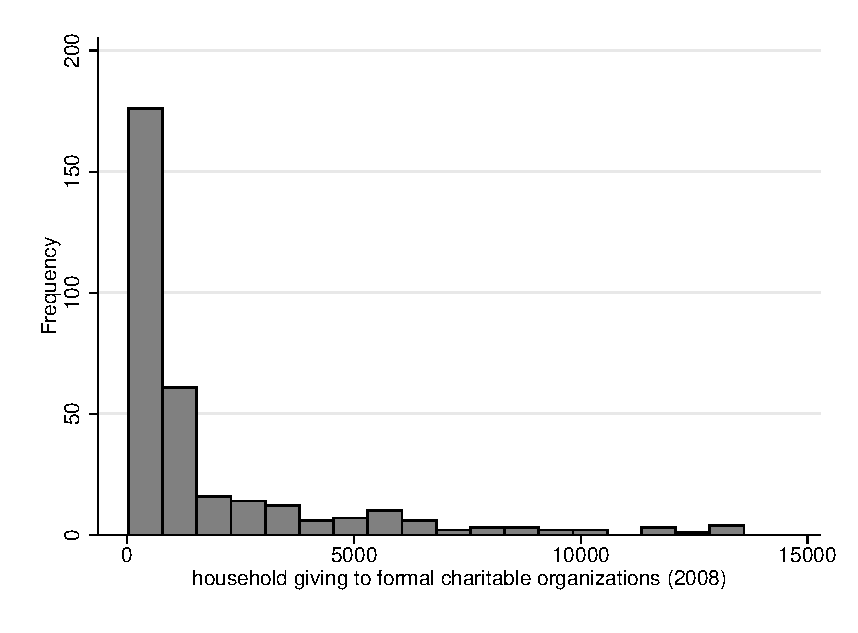
\includegraphics[angle=0,
           width=.75\textwidth]{gave.eps}
   \caption{Distribution of charitable giving}
  \label{fig:gave}
\end{figure}
\begin{table}[htbp]
\caption{\label{tab:charitydes} Summary statistics for charity models}\centering\medskip
\begin{tabular}{llcc}\hline
Variable & Description & $mean$ & $SE\left(mean\right)$  \\ \hline
gaveamt & Amount given & 1796.99 & 148.64 \\
hhincome & Income in k & 60.36 & 1.20 \\
lngaveamt & ln(Amount given) & 6.54 & 0.08 \\
lnhhincome & ln(Income in k) & 4.02 & 0.02 \\ \hline
 \end{tabular}
\end{table}
When we examine our outcome, amount given, we see that it is highly skewed, see Figure~\ref{fig:gave}. This will most likely produce several problems:
\begin{enumerate}
\item The variance will not be constant
\item The mean of the residuals will not consistently be zero
\item We may have outliers in the tail of the distribution
\end{enumerate}


\begin{table}[htbp]\centering
\caption{ Models predicting charitable giving in dollars
\label{tab:charity}}
\begin{tabular}{lcccc}
\hline
Coefficients&Model 1&Model 2&Model 3&Model 4 \\ \hline
hhincome centered  &   22.614*** &    0.014*** &        &        \\
      &   (6.777)  &   (0.004)  &        &        \\
ln(hhincome) centered &        &        &  1156.648** &    0.730*** \\
      &        &        &  (356.840)  &   (0.193)  \\
Intercept    &  1796.988*** &    6.543*** &  1796.988*** &    6.543*** \\
      &  (146.392)  &   (0.079)  &  (146.528)  &   (0.079)  \\
\hline
\multicolumn{5}{l}{Model Statistics} \\
\hline
$N$ &   328.000  &   328.000  &   328.000  &   328.000  \\
$F$ 	 &   11.134  &   14.822  &   10.506  &   14.296  \\
$R^2$  &    0.033  &    0.043  &    0.031  &    0.042  \\
$df$ Regression &    1.000  &    1.000  &    1.000  &    1.000  \\
$df$ Error 		 &   326.000  &   326.000  &   326.000  &   326.000  \\
Log-likelihood &  -3049.966  &  -582.776  &  -3050.271  &  -583.030  \\
\hline
\multicolumn{5}{l}{Models 2 and 4 have a logged outcome. hhincome in thousand dollar units.} \\
\multicolumn{5}{l}{$SE$s in parentheses, $***p<0.001$} \\
\hline
\end{tabular}
\end{table}
Table~\ref{tab:charity} presents four models. The first model predicts giving with income using the unaltered versions of both variables (note: income is centered):
\[
gave_i=\beta_0+\beta_1\left(hhincome_i-\overline{hhincome}_i\right) + e_i.
\]
The second model predicts the natural log of giving with the unaltered version of income:
\[
\mbox{ln}\left(gave_i\right)=\beta_0+\beta_1\left(hhincome_i-\overline{hhincome}_i\right)+e_1.
\]
The third model predicts unaltered giving with the natural log of income, centered on the mean natural log of income:
\[
gave_i=\beta_0+\beta_1\left(\mbox{ln}\left(hhincome\right)_i-\overline{\mbox{ln}\left(hhincome\right)}_i\right) + e_i.
\]
Finally, the fourth model predicts the natural log of giving with the natural log of income, centered as well:
\[
\mbox{ln}\left(gave_i\right)=\beta_0+\beta_1\left(\mbox{ln}\left(hhincome\right)_i-\overline{\mbox{ln}\left(hhincome\right)}_i\right)+e_i.
\]
\paragraph{Interpretation of Model 1}

Since we centered income, the intercept indicates that a household with average income gives about 1,797 dollars. For each thousand dollars increase in income, giving increases by about 23 dollars. Overall, this model explains about 3.3 percent of the variation.

\paragraph{Interpretation of Model 2}

In this model, we have transformed giving into the natural log of giving. Income is still centered, so the intercept is still the average natural log of giving. We can take the exponent of this quantity to estimate the geometric mean of giving (not the arithmetic mean)
\begin{equation}
e^{\beta_0} = \left(\bar{y}_{geometric}|x=0\right)
\end{equation}
\[
e^{6.543} = 694.37
\]
which tells us that the average household gives about 694 dollars. This estimate is much smaller than Model 1 (1,797 dollars).

Estimating the effect of income requires us to take the exponent of $\beta_1$. Thus, $\left(e^{\beta_1}-1\right)\times100$ will tell us the percent increase in the outcome for a one unit change in the predictor if $\beta_1>0$. When $\beta_1<0$, $\left(1-e^{\beta_1}\right)\times100$ will tell us the percent decrease in the outcome for a one unit change in the predictor. For example, when income is at the mean, we have already established that the amount given is 694.37 dollars. If we increase income by a thousand dollars (a one unit increase), the dollar amount given is
\[
e^{6.543+0.014} = 704.16
\]
The ratio of these two amounts is
\[
\frac{y|x=1}{y|x=0} = \frac{704.16}{694.37}=1.014
\]
which is equal to the exponent of the slope
\[
e^{\beta_1}=\frac{y|x=1}{y|x=0}
\]
\[
e^{0.014}=1.014
\]
which indicates a
\[
\left(e^{\beta_1}-1\right)\times100 = \left(1.014-1\right)\times100=1.4 \mbox{ percent}
\]
increase. Note that the fact that the coefficient was 0.014 and the percent increase was 1.4 is a coincidence. When the coefficient is larger, the numbers will not match.

If we log these variables, their distributions behave better (but what we really care about is the distribution of giving)

\paragraph{Interpretation of Model 3}

We know that the average donation for the log of the average household income is 1,796.99. What does the coefficient mean? To understand that we need to realize that since we logged our predictor, our comparison is between the average log and an additional log. This would be a lot of income. Let's instead say that income increases 10 percent (or by a factor of 1.1). This makes the difference in our outcome as
\[
1156.648\times\mbox{ln}\left(1.1\right)=110.24 \mbox{ dollars}
\]

The final use of log-transformations in OLS regression is when both dependent and predictor variable are logged.

\paragraph{Interpretation of Model 4}

In this model, both the outcome and predictor is transformed to the natural log. This produces an elasticity. Thus, coefficient tells us the percent ({\it not proportion}) change in the outcome based on a 1 {\it percent} change in the predictor. Here, we see that giving changes by 0.730 percent, for each percentage change in the predictor. Here is a walk-through on how this works.

Table~\ref{tab:charitydes} gives the means for our variables, both the unaltered version and the natural log version. From Table~\ref{tab:charity}, we can find that the dollar amount for the mean natural log of giving is $e^{6.543}=694.37$ dollars. The mean natural log of income is 4.02, which translates into an amount of $e^{4.02}=55.70$ thousand dollars. A 1 percent increase of 55.70 thousand dollars is $1.01\times55.70 = 56.26$ thousand dollars, of which the natural log is 4.03. Thus, a 1 percent increase in the natural log of income is 0.01. Plugging this into the model, our predicted natural log of giving is $6.543+0.730\left(0.01\right)=6.550$, the exponent of which is 699.45. $\left(699.45 - 694.37\right)/694.37=0.01$, or a 1 percent increase.

\subsubsection{Testing models with log likelihoods}
\label{sec:likelihoodtest}
As a bonus, Table~\ref{tab:charity} includes the log likelihood of each model. We can only compare log likelihoods for models with the same outcome and exact same set of data. That means we can compare Models 1 and 3, and Models 2 and 4.

Recall that the log likelihood of a model is $\mbox{ln}\left(L\left(\theta\right)\right)$. Also remember that the test of two log likelihoods for models A and B is equation~\eqref{eq:lrtest}
\[
\chi^2=2\left(\mbox{ln}\left(L\left(\theta_a\right)\right)-\mbox{ln}\left(L\left(\theta_{null}\right)\right)\right)
\]
We see the log likelihood of Model 1 in Table~\ref{tab:charity}, the model with unaltered predictors with the unaltered outcome, is -3029.966, and the likelihood of Model 3, the model with the natural log of income with the unaltered outcome is -3050.271. The test comparing whether Model 3 is a better model is
\[
\chi^2=2\left(-3029.966- -3050.271\right)=40.61
\]
We can then evaluate this against the $\chi^2$ distribution with 1 degree of freedom, which produces a probability of 0.000000002. This is clear evidence that using the unaltered version of the predictor, Model 1, is a much better model. Looking at Models 2 and 4, this test results in 0.508, the probability of which is 0.476, telling us that there is no difference, statistically, in the model fit between Models 2 and 4.

\section*{For more information}
For comprehensive treatment of variable coding and transformation strategies in regression, see \citep{fox} and \citep{hill}. For discussion of logarithmic transformations and elasticity interpretations, consult \citep{cameron2005microeconometrics}. Maximum likelihood methods and likelihood ratio testing are covered in detail in \citep{eliason1993maximum}.